\cleardoublepage
\chapter{Introduction\label{ch:introduction}}

\section{The many-electron problem}
In materials science, all the properties of a given system whether, they are mechanical, chemical, or optical, can be explained in terms of the fundamental interactions between their elemental components: electrons and nuclei. At a good level of approximation, where only relativistic and hyperfine effects are neglected, all these interactions are embodied in the following Hamiltonian (given in atomic units):
%
\begin{equation}
    \hat{H}_{tot} = - \sum_I \frac{\nabla_I^2}{2M_I} - \sum_i \frac{\nabla_i^2}{2} + \sum_{i < j} \frac{1}{|\br_i - \br_j|} - \sum_{i,I} \frac{Z_I}{|\br_i - \bR_I|} + \sum_{I < J} \frac{Z_I Z_J}{|\bR_I - \bR_J|} ,
    \label{eq:many-body}
\end{equation}
%
where the first two terms represent, respectively, the kinetic energies of the nuclei ($\hat{T}_N$) and of the electrons ($\hat{T}$), and the following three terms embed their individual and reciprocal electrostatic interactions -- $\hat{V}_{\rm ee}$, $\hat{V}_{\rm eN}$, and $\hat{V}_{\rm NN}$. The complexity of the problem is drastically reduced when the \emph{Born-Oppenheimer approximation} is applied \cite{born_zur_1927}: based on the observation that the electronic mass is much smaller than the mass of the ions ($m_e / M_I \thicksim 10^{-3} - 10^{-5}$), the rotation period of the electrons is way shorter than the vibration period of the nuclei, to the point that the latter can be considered steady from an electronic point of view. The electronic and nuclear dynamics can then be decoupled and described in terms of two distinct Schr\"{o}dinger equations. The electrons interact within the field generated by the frozen nuclei thereby the (electronic) Hamiltonian, $\hat{H}_{\rm e}$, includes the electron-electron repulsion and the nuclear potential $V(\br,\{ \bR_I \})$ where the positions $\bR_I$ are treated as parameters. The associated Schr\"{o}dinger equation reads as
%
\begin{equation}
    \underbrace{\left( \hat{T} + \hat{V}_{\rm ee} + \hat{V}(\{ \bR_I \}) \right)}_{\hat{H}_{\rm e}} \Psi_n(\{ \bR_I \}) = E_n(\{ \bR_I \}) \Psi_n(\{ \bR_I \}) .
    \label{eq:many-electron-problem}
\end{equation}
%
The electronic energies $E_n(\{ \bR_I \})$ play the role of potential energy surfaces for the nuclei and, by taking the lowest of them, we obtain the nuclear Schr\"{o}dinger equation:
%
\begin{equation}
    \left( \hat{T}_{\rm N} + E_0(\{ \bR_I \}) \right) \Phi_n = W_n \Phi_n ,
    \label{eq:nuclear-schrodinger-eq}
\end{equation}
%
whose solutions yield all the properties of the nuclear system, including the \emph{phonon modes}.

Thanks to the Born-Oppenheimer approximation, \cref{eq:many-body} gets split into two ``simpler'' problems: one -- \cref{eq:many-electron-problem} -- defining the electronic structure of the system, the other -- \cref{eq:nuclear-schrodinger-eq} -- determining the motion of the nuclei. The two problems are radically different, meaning that the methods developed to search for their solutions are not the same. Here, we are interested in the solution of the electronic Hamiltonian, whereas the problem of the dynamics of the nuclei is out of the scopes of this work. Nevertheless, it is important to mention that the effects due to the coupling between the electron and the nuclear dynamics are not always negligible, and the nuclear motion can actually influence the electronic structure of a material. Ground- and excited-state energies, including the fundamental gap, can be significantly affected and demand for a treatment of the electron-phonon coupling. While the theory behind the renormalization effects of the electronic structure will not be discussed here, the corrections that account for them will be included (when needed) in the presented results.

\section{First-principles electronic-structure methods\label{sec:first-principles-methods}}
Except for a bunch of very special and strongly unrealistic systems, the Hamiltonian of a set of interacting electrons cannot be solved exactly. Many methods, grounding on fundamentally different strategies, have been developed in order to tackle the many-electron problem, some of them dating back to more than sixty years ago. However, it is only in the last few decades that the computing power has reached a level that allowed for an effective use of these methods in computational materials science. Most of the methods used today follow the idea of the first-principles, or \emph{ab initio}, approach, where the solution of the problem is determined by starting from the fundamental laws of physics -- i.e. the Schr\"{o}dinger equation \eqref{eq:many-electron-problem} -- without introducing any empirical fitting or model.

First-principles methods for electronic-structure calculations can be divided in three big categories, depending on the type of descriptor chosen to characterize the system: the many-body wave function $\Psi(\br_1, \dots, \br_N)$, the total density $\rho(\br)$, or the Green's function $G(\br,t,\br',t')$ \cite{marzari_electronic-structure_2021}. Each strategy concentrates the complexity of the problem on a different aspect, which brings to different advantages and drawbacks.

Historically, the wave function is the descriptor favored by the chemistry community, from which the name \emph{quantum chemistry methods} to classify the approaches that follow this road. Essentially, all the approximations are usually done on the electronic wave function whereas the Hamiltonian of \cref{eq:many-electron-problem} is taken in its exact form. Among the first and simplest examples we find the Hartree-Fock system \cite{hartree_wave_1928,fock_naherungsmethode_1930}, where the wave function is approximated to a single Slater determinant, which accounts correctly for the exchange energy (a form of interaction deriving from the fermionic character of the electrons), but misses completely the electronic correlation. By improving the sampling of the wave function -- namely combining several, wisely chosen, Slater determinants -- the quality of results tends to increase together with the computational cost of a calculation. Quantum chemistry methods provide the most accurate predictions of many ground-state and excited-state properties, with a precision that often exceeds that of ``rival'' methods of several orders of magnitudes; nevertheless, this is combined with the worst scaling properties with respect to the system size, which usually limits the use of these approaches only to small molecules.

An alternative formulation of the many-electron problem rose up when, in 1964, Hohenberg and Kohn (HK) discovered the fundamental connection that links the ground-state density of a system to the Hamiltonian \cite{hohenberg_inhomogeneous_1964}, and thus to any of its properties, giving birth to density-functional theory (DFT). All the physical observables, starting from the total energy, are functionals of the ground-state density -- an object depending only on one spatial coordinate, thus infinitely simpler than the many-body wave function -- which, in principle, determines univocally all the properties of the system. Unfortunately, while the HK theorem proves the existence of such connection, it does not provide any information about the explicit dependence of the energy (or other quantities) on the density: it is the search for such mathematical relations, or better, of a reliable approximation to them, that represents the main challenge of DFT. Despite the breakthrough brought about by this theory, it was only twenty years later, when the first approximations of the unknown exchange and correlation (xc) energy functional started to come out, that DFT became a practical tool. Since then, the use of DFT exploded, and today it represents the most widely employed method for electronic-structure calculations, as confirmed by the presence of twelve DFT-based papers in the list of the hundred most cited papers of all times (as of 2014), including two in the top-10 \cite{van_noorden_top_2014}.

Finally, we have the class of methods that rely on the one-particle Green's function of the system, which fulfills the role of electron (and hole) space-time propagator. The Green's function is a non-local object -- both in space and time -- that provides direct access to many important properties of the system, including the electron addition and removal energies. Determining the Green's function of the system is the goal of this approach; this can be done via many-body perturbation theory (MBPT), a theory which grounds its roots on the definition of the Green's function as a series expansion in terms of the Coulomb interaction. Such expression can be recast into a non-linear Dyson equation for the Green's function, where the complexity of the perturbative expansion is moved into a dynamical effective interaction called self-energy. Computing the self-energy -- again, by converging a series of Coulomb-like integrals -- is not an easier task; however, in 1965, Hedin introduced a closed set of equations that connect the Green's function and the self-energy to other three quantities -- namely the screened interaction, the electric polarizability, and the vertex function -- and whose solution can be obtained in self-consistent manner \cite{hedin_new_1965}. The infamous \gw approximation results from the first loop over Hedin's equations, and represents one of the most successful applications of Green's function theory for the study of the properties of materials.

If we put aside the wave function-based methods -- here the improvements consist in a better sampling of the wave function which usually involves the rigorous, yet computationally inefficient, increase of the size of the basis set -- current research in electronic-structure methods aims to improve the capabilities of DFT and Green's function-based approaches. In Green's function theory, this often involves: (i) a more suitable choice for the one-electron states used within the definition of, e.g., $G$ \cite{bruneval_benchmarking_2013}, and (ii) better expressions for the quantities involved in the Hedin's loop -- by improving, e.g., the approximation on the vertex yielding the \gw approximation ($\Gamma=\delta \delta$) \cite{chen_accurate_2015}. In DFT instead, the improvements usually affect the xc functional. The Jacob's ladder of density-functional approximations depicts the gap that separates the Hartree world (zeroth-order approximation) from the heavenly chemical accuracy, and where the current types of approximation sit \cite{perdew_jacobs_2001}. Starting from the local-density approximation, the accuracy grows when additional features are included in the functional. In this way, one goes from GGA and meta-GGA, which include the derivatives of the density (and sometimes the kinetic-energy densities), to non-local approaches where the exchange and, ultimately, the correlation, are expressed in terms of the one-particle wave functions rather than the density. With the increasing accuracy, also the computational costs grow, thus it is the compromise of the two best fitting a given calculation that defines the optimal approximation.

\begin{figure}
    \centering
    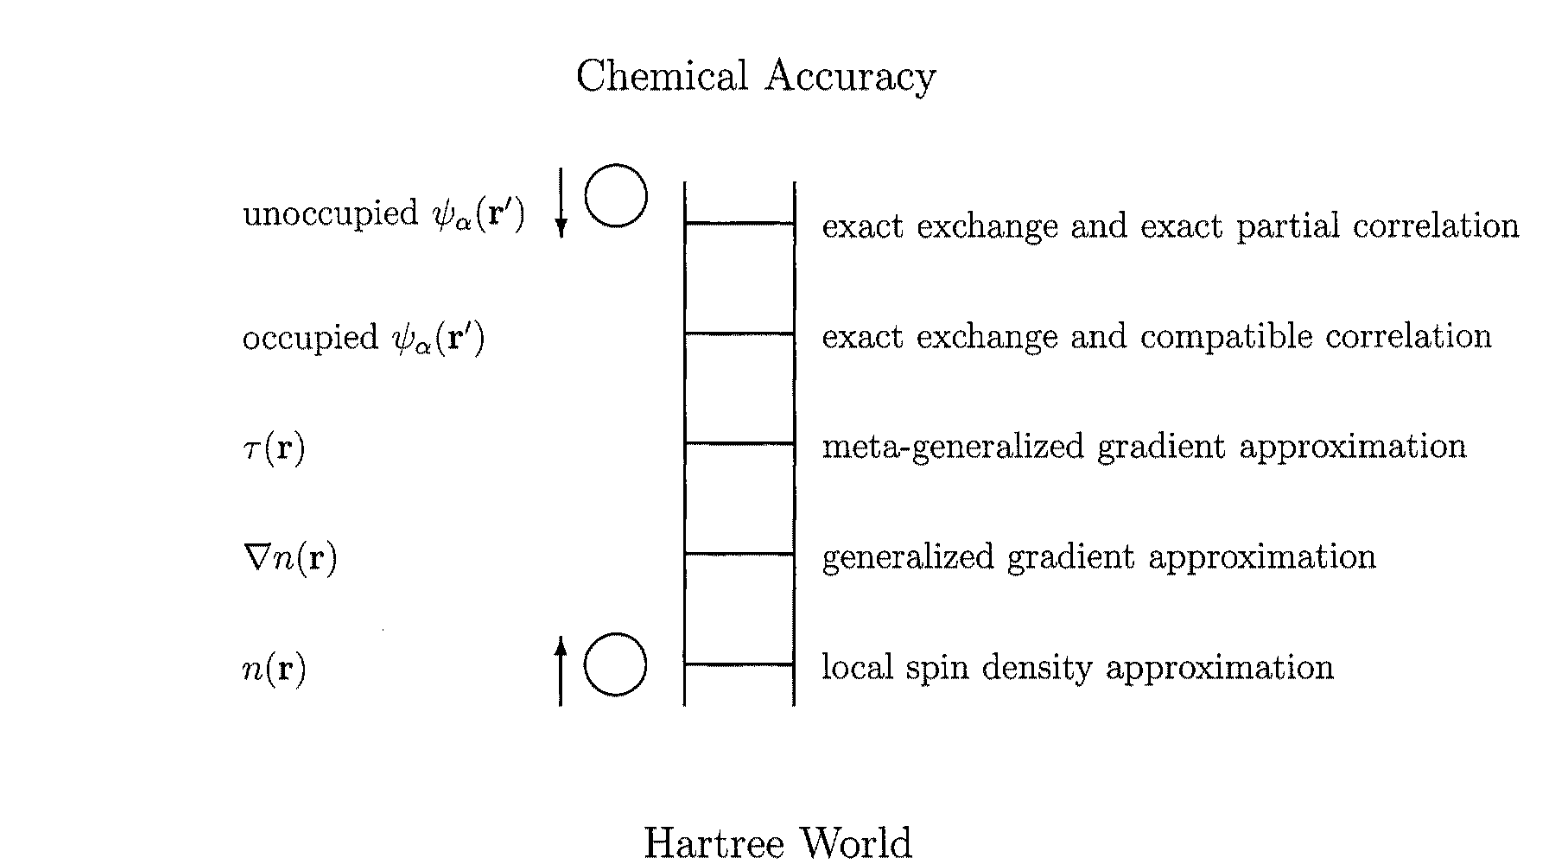
\includegraphics[width=\linewidth]{jacob-ladder.png}
    \caption[Jacob's ladder for density-functional approximations]{Jacob's ladder for density-functional approximations; figure taken from Ref.~\cite{perdew_jacobs_2001}.}
    \label{fig:jacob-ladder}
\end{figure}

Besides the quality of the approximations used, another important aspect regards which properties (and with what effort) can be predicted by either of the two approaches. While DFT is the ideal approach for the computation of ground-state densities and energies (and derived quantities), with respect to spectral properties, Green's function theory is naturally more suitable, since it provides almost directly the photoemission and absorption spectra of materials. Although these properties are determined, in principle, by the ground-state density, the explicit expression in terms of $\rho$ is not known (and it is not guaranteed to exist!), which explains why it is so difficult to extract the information about the spectral properties in a DFT framework. The Kohn-Sham (KS) mapping defines an auxiliary system of non-interacting electrons that shares the same ground-state density of the real system. However, the interpretation of the KS eigenvalues as quasiparticle energies is not supported by the theory (except for the highest-occupied energy level which matches the actual ionization potential), and usually one has to relax the constraints imposed by KS-DFT in order to capture the physics of charged and neutral excitations. Part of the problem comes from the fact that the interaction ``felt'' by an electron is represented by the (dynamical and non-local) self-energy, whereas the KS effective potential is a local and static object which is uncapable of tracing the interactions resulting at different spaces and times.

Designing an approach whose effective interaction embodies part of these features while preserving the computational feasibility of DFT, represents then one of the possible strategies to tackle spectral properties of materials, and it is where Koopmans spectral functionals find their way in the landscape of electronic-structure methods.

\section{Koopmans spectral functionals\label{sec:intro-koopmans}}
Koopmans spectral functionals represent a novel approach for the calculation of charged excitations, grounding on a DFT-based framework. The goal of Koopmans functionals, is that of defining a mean-field approach where single-particle states fulfill the role of quasiparticles. In this context, the eigenvalues of the effective one-particle Hamiltonian provide the peaks of the direct, and inverse, photoemission spectra. All this is done in the formalism of energy functionals, where one can take advantage of the variational principle to determine the ground-state of the system. Behind the construction of Koopmans functionals there is the exact property of the ground-state energy of being a piecewise-linear function with respect to the number of electrons \cite{perdew_density-functional_1982}. Such property is generally not satisfied by standard density-functional approximations which exhibit an unnatural non-linear trend, creating a discrepancy between total and differential energy differences. The idea behind Koopmans functionals is that of imposing the piecewise-linearity condition, but in a more restrictive form: this is not simply applied to the energy as a function of the number of electrons, but it is actually extended to the occupations of all the orbitals in the system. The imposition of such generalization of the piecewise-linearity condition defines a framework that restores the correspondence between total energy differences and energy derivatives, with the latter corresponding to the eigenvalues of an effective Hamiltonian. In other words, it brings to an approach where the Koopmans theorem \cite{koopmans_uber_1934} is satisfied.

Any Koopmans functional starts from some simple density-functional approximation (usually local or semi-local functionals), and makes it compliant with the aforementioned generalized piecewise-linearity condition. Inevitably, this brings to a functional which depends explicitly on the individual orbital densities, and breaks the invariance of the energy with respect to unitary transformations. Notwithstanding the inevitable increase of complexity with respect to standard density-functionals, the orbital-density-dependence brings about some features typical of the dynamical self-energy, and hints at the interpretation of Koopmans potentials as approximated many-body potentials \cite{ferretti_bridging_2014}.

In the past years, Koopmans functionals have been applied successfully for the calculation of spectral properties of finite systems. Among the most relevant applications of Koopmans functionals, we recall the predictions of the photoemission spectra of the DNA and RNA molecules \cite{nguyen_first-principles_2016}, and of liquid water \cite{de_almeida_electronic_2021}. The reduced computational cost, when related to other spectral approaches, goes along with the high accuracy, comparable to that of state-of-the-art MBPT methods \cite{colonna_koopmans-compliant_2019}. In extended systems, Koopmans functionals confirmed their high predictive power \cite{nguyen_koopmans-compliant_2018,de_gennaro_blochs_2022,colonna_koopmans_2022}, as showed also in this thesis, establishing themselves among the best methods for the calculations of photoemission properties of materials.

\section{Objectives\label{sec:objectives}}
The goal of this thesis is to consolidate, both conceptually and technically, the applications of Koopmans spectral functionals in extended systems. Among the difficulties affecting calculations in extended systems, is the requirement of a set of localized orbitals in order to have effective Koopmans corrections. A localized representation of the orbitals opposes the Bloch-wave form of the one-electron states propagating in a periodic system, and hinders the validity of Bloch's theorem. Indeed, because of the orbital-density-dependent character of Koopmans functionals, the potentials built on localized -- thus non-periodic -- orbital-densities are also non-periodic over the system's primitive cell, and generally break the translation symmetry of the system. In a scenario where Bloch's theorem does not apply, the description of the quasiparticle spectrum via a band structure picture is not possible.

For a crystalline material, the set of translations along all the vectors of the underlying Bravais lattice represent a symmetry group. As a consequence, the band structure -- i.e. the $\bk$-resolved description of the energy spectrum -- is a natural way of representing the one-particle excitation energies, and constitutes an actual observable that can be measured by means of an angle-resolved photoemission (ARPES) experiment \cite{damascelli_angle-resolved_2003}. A computational experiment must be able to provide this information, that is why in this thesis we address the problem of the validity of Bloch's theorem in the framework of Koopmans functionals (and, more generally, of orbital-density-dependent functionals).

Besides the proof-of-concept, the computation of the band structure requires to develop an unfolding technique, able to reconstruct the $\bk$-dispersion relation of the energy from a supercell calculation (the latter, is still necessary in order to ensure the localization of the orbitals). Part of the work of this thesis, was then devoted to the development of an unfolding method. 
Additionally, a lot of effort was put to improve the computational code to perform calculations with Koopmans functionals.

\section{Organization of the thesis\label{sec:organization-thesis}}
The thesis is organized as follows.

In \textbf{\cref{ch:theoretical-background}}, we describe the theoretical background underlying electronic-structure calculations, with a particular focus on spectral properties. We start from DFT and briefly discuss the main aspects of the theory, pointing out the limitations affecting this approach both at an exact level and in standard approximations. We then move to non-local methods, where we highlight the advantages of embodying the exact exchange in the expression for the exchange-correlation functional. Finally, we discuss the main features of Green's function-based methods, with a particular emphasis on the dynamical nature of the effective electronic interaction.

In \textbf{\cref{ch:koopmans-theory}}, we introduce Koopmans functionals. Starting from the idea behind the generalized piecewise-linearity condition, we describe how Koopmans corrections are realized and how the ground-state of orbital-density-dependent functionals is determined. A specific section is devoted to the recent definition of the Koopmans Hamiltonian, an important aspect that turned out to be very useful to show the compliance of Koopmans functionals with Bloch's theorem. In the second part of the chapter, we discuss the connection between Koopmans functionals and many-body perturbation theory.

\textbf{\cref{ch:koopmans-periodic}} is devoted to the central result of this thesis, i.e. the validity of Bloch's theorem in orbital-density-dependent functionals. We start the chapter describing the importance of having a set of localized orbitals when performing calculations in extended systems. Then we discuss Bloch's theorem, and how this applies to standard density-functional approaches and to orbital-density-dependent methods. Finally, we give an overview of a recent implementation of Koopmans functionals, which exploits the compliance with the translation symmetries of the system to develop a primitive cell-based approach.

In \textbf{\cref{ch:band-structures}}, we discuss the band structure calculations performed on a set of benchmark semiconductors and insulators. The chapter opens with a description of the unfolding method and of the workflow to run calculations with Koopmans functionals. A small section is also dedicated to the finite-size corrections used when performing calculations on charged cells. In the second part, we report and discuss the results obtained with the two implementations of Koopmans functionals.

In \textbf{\cref{ch:defects}}, we introduce a new application that we considered recently, i.e. the impurity energy levels in semiconductors rising upon the presence of point defects. We outline the strategies that we devised to tackle the problem, and we report the preliminary results that we obtained for the arsenic-antisite defect in gallium arsenide.

The thesis is closed by a section of \textbf{Conclusions}, where we summarize the main messages of this thesis, and give an overview of the possible future developments.
